\documentclass[12pt]{standalone}

\usepackage{tikz}


\begin{document}
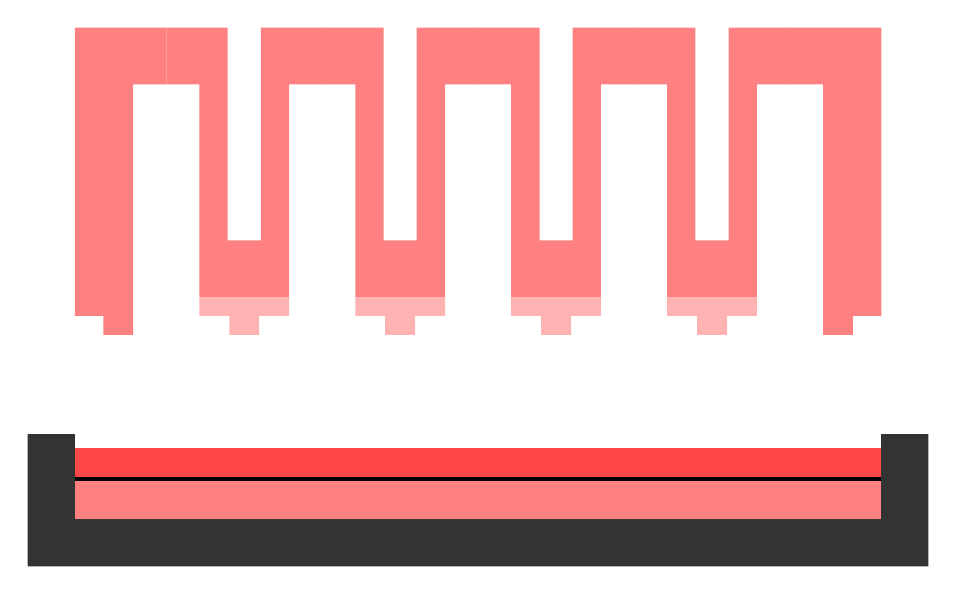
\begin{tikzpicture}[scale=.6,
kontur/.style={black, very thick},
konturback/.style={thick},
elastosil/.style={fill=red!50},	% geschnittenes Elastosil
elaback/.style={fill=red!30},	% Elastosil im Hintergrund
flussig/.style={fill=red!80, opacity=1},	% flüssiges Elastosil
flussigg/.style={fill=red!90, opacity=.8},	% flüssiges Elastosil
nichtdehnbar/.style={fill=black},	% Papierstreifen 
schrift/.style={black, thin},
housing/.style={fill=black!80}
]

%%%%%%%%%%%%%%%%%%%%%%%%%%%%%%%%%%%%%%%%5


% Defs of Basis

\def\hy{4.5}		% Höhe y
\def\hx{1}		% Halbe Höhe x
\def\xl{1.3}		% x distance luecke
\def\thick{.3}	% Halbe Dicke
\def\hya{.4}	% Höhe y Absatz
\def\hyl{.8}	% Höhe Luftkanal		
\def\N{5}		% Anzahl Kammern

% Defs of Bottom

\def\bhy{.8}		% Höhe Boden
\def\bdy{.1}		% Abstand zwischen Basis und Boden
\def\fhy{.6}		% Höhe ElastosilLevel


% Defs of Schnitt

\def\xshift{18}
\def\sxges{6}


% Implicite
\pgfmathsetmacro{\xges}{\hx+\hx+\xl}
\pgfmathsetmacro{\xgesh}{\xges/2}
\pgfmathsetmacro{\yges}{\hy+\hyl}
\pgfmathsetmacro{\hxa}{(\xl+\thick+\thick)/3}
\pgfmathsetmacro{\X}{\xges*(\N-2)}
\pgfmathsetmacro{\Xges}{\X+\xges+2*\thick+2*\hxa+2*\hx}
\pgfmathsetmacro{\bhyh}{\bhy/2}
\pgfmathsetmacro{\shx}{1/4*(\sxges-5*\hxa-4*\thick)}



%%%% HOUSING
%
%\path[housing] (-\hx-\thick-\hxa,-3*\thick-\yges)++(-1,-.5)--++(\Xges+2, 0)--++(0,\yges+4*\thick+.5)--++(-2-\Xges, 0)--cycle;
%


%%%%%%%%%%%%%%% BASIS %%%%%%%%%%%%%%%%%%

\foreach \x[count=\i] in {0, \xges, ..., \X}{

\path (\x,0)coordinate(OL); 	% Koord oeben links
\path (OL)++(\xges,-\thick-\thick-\thick)coordinate(B);
\def\konturOben{
(OL)++(0,\thick)--++(\hx+\thick,0)--++(0,-\hy)--++(\xl-\thick-\thick,0)--++(0,\hy)--++(\hx+\thick,0)coordinate(OR)
}
\def\konturUnten{
(B)
--++(-\hx+\thick,0)
--++(0,-\hy)coordinate(UR)
--++(-\xl-\thick-\thick,0)coordinate(UL)coordinate[midway](Luftkanal\i)
--++(0,\hy)
--++(-\hx+\thick,0)
}
\def\konturBack{
(UL)
--++(0,-\hyl+\hya)
--++(\hxa,0)
--++(0,-\hya)
--++(\hxa,0)coordinate[midway](Absatz\i)
--++(0,\hya)
--++(\hxa,0)--(UR)}

\path \konturUnten; % Just for defining the nodes

%% Elastosil
\path[elaback] \konturBack;
\path[elastosil] \konturOben -- \konturUnten;

}

%%%%%%%%%%%%%%% FlUEssig %%%%%%%%%%%%%%%%%%

%\path[flussig] (-\hx-\thick-\hxa,-\yges-\bdy-\thick-\thick-\thick) rectangle ++(\Xges,\fhy)coordinate[midway](Flussig);


%% Enden
\def\konturEndeRechts{
(B)
--++(\hx-\thick,0)
--++(0,-\yges)
--++(\hxa,0)coordinate[midway](Lippe)
--++(0,\hya)
--++(\thick+\thick,0)
--++(0,\yges-\hya+4*\thick)--(OR)}
\path[elastosil] \konturEndeRechts;



\def\konturEndeLinks{
(0,-\thick-\thick-\thick)--++(-\hx+\thick,0)--++(0,-\yges)--++(-\hxa,0)coordinate(help)--++(0,\hya)--++(-\thick-\thick,0)--++(0,\yges-\hya+4*\thick)--(0,\thick)}
\path[elastosil] \konturEndeLinks;

\path[draw] (help)++(-\thick-\thick,-\bdy)coordinate(BOL);





%%%%%%%%%%%%%% Boden %%%%%%%%%%%%%%%%%%%%%%%%%%

\path[elastosil] (BOL)++(0,-3)coordinate(BOL)--++(\Xges,0)--++(0,-\bhy)coordinate(BUR)--++(-\Xges,0)--cycle;

\path[housing] (BOL)--++(0,1)--++(-1,0)--++(0,-1-\bhy-1)--++(2+\Xges,0)--++(0,2+\bhy)--++(-1,0)--++(0,-1-\bhy)--++(-\Xges,0)--cycle;

\path[nichtdehnbar] (BOL)rectangle++(\Xges,.1)coordinate(nichtDehnbar);
\path[flussigg] (nichtDehnbar)rectangle++(-\Xges,\fhy);



\end{tikzpicture}
\end{document}